%%%%%%%%%%%%%%%%%%%%%%%%%%%%%%%%%%%%%%%%%
% Beamer Presentation
% LaTeX Template
% Version 1.0 (10/11/12)
%
% This template has been downloaded from:
% http://www.LaTeXTemplates.com
%
% License:
% CC BY-NC-SA 3.0 (http://creativecommons.org/licenses/by-nc-sa/3.0/)
%
%%%%%%%%%%%%%%%%%%%%%%%%%%%%%%%%%%%%%%%%%

%----------------------------------------------------------------------------------------
%	PACKAGES AND THEMES
%----------------------------------------------------------------------------------------

\documentclass{beamer}

\mode<presentation> {

% The Beamer class comes with a number of default slide themes
% which change the colors and layouts of slides. Below this is a list
% of all the themes, uncomment each in turn to see what they look like.

%\usetheme{default}
%\usetheme{AnnArbor}
%\usetheme{Antibes}
%\usetheme{Bergen}
%\usetheme{Berkeley}
%\usetheme{Berlin}
%\usetheme{Boadilla}
% \usetheme{CambridgeUS}
%\usetheme{Copenhagen}
%\usetheme{Darmstadt}
%\usetheme{Dresden}
%\usetheme{Frankfurt}
%\usetheme{Goettingen}
%\usetheme{Hannover}
%\usetheme{Ilmenau}
%\usetheme{JuanLesPins}
%\usetheme{Luebeck}
\usetheme{Madrid}
%\usetheme{Malmoe}
%\usetheme{Marburg}
%\usetheme{Montpellier}
% \usetheme{PaloAlto}
%\usetheme{Pittsburgh}
%\usetheme{Rochester}
%\usetheme{Singapore}
%\usetheme{Szeged}
%\usetheme{Warsaw}

% As well as themes, the Beamer class has a number of color themes
% for any slide theme. Uncomment each of these in turn to see how it
% changes the colors of your current slide theme.

%\usecolortheme{albatross}
%\usecolortheme{beaver}
%\usecolortheme{beetle}
%\usecolortheme{crane}
%\usecolortheme{dolphin}
%\usecolortheme{dove}
%\usecolortheme{fly}
%\usecolortheme{lily}
%\usecolortheme{orchid}
\usecolortheme{rose}
%\usecolortheme{seagull}
%\usecolortheme{seahorse}
%\usecolortheme{whale}
%\usecolortheme{wolverine}

%\setbeamertemplate{footline} % To remove the footer line in all slides uncomment this line
%\setbeamertemplate{footline}[page number] % To replace the footer line in all slides with a simple slide count uncomment this line

%\setbeamertemplate{navigation symbols}{} % To remove the navigation symbols from the bottom of all slides uncomment this line
}

\usepackage{graphicx} % Allows including images
\graphicspath{{./fig/}}
\DeclareGraphicsExtensions{.pdf,.jpeg,.png}
\usepackage{booktabs} % Allows the use of \toprule, \midrule and \bottomrule in tables
\usepackage[numberedbib]{apacite}
\usepackage{ amssymb }

%----------------------------------------------------------------------------------------
%	TITLE PAGE
%----------------------------------------------------------------------------------------

\title[ContCtrl with deepRL (Lilicrap, 2016)] {
    Continuous control with deep reinforcement learning
    \vspace{5mm}
    (DeepRL Reading, RDL, UQ)
}

\author{Vektor Dewanto} % Your name
\institute[RDL, UQ] % Your institution as it will appear on the bottom of every slide, may be shorthand to save space
{
% Affiliation: RDL, UQ\\ % Your institution for the title page
\medskip
\textit{vektor.dewanto@gmail.com } % Your email address
}
\date{\today} % Date, can be changed to a custom date

\begin{document}

\begin{frame}
\titlepage % Print the title page as the first slide
\end{frame}

\begin{frame}
\frametitle{Outline} % Table of contents slide, comment this block out to remove it
\tableofcontents % Throughout your presentation, if you choose to use \section{} and \subsection{} commands, these will automatically be printed on this slide as an overview of your presentation
\end{frame}

%----------------------------------------------------------------------------------------
%	PRESENTATION SLIDES
%----------------------------------------------------------------------------------------
%%%%%%%%%%%%%%%%%%%%%%%%%%%%%%%%%%%%%%%%%%%%%%%%%%%%%%%%%%%%%%%%%%%%%%%%%%%%%%%
\section{Introduction}
\frame{\tableofcontents[currentsection, hideothersubsections]}

\begin{frame}
\frametitle{Introduction}
Problems:
\begin{itemize}
  \item continuous action space
  \item raw pixels for observations
\end{itemize}
\vspace{5mm}

DDPG (=DPG+DQN)~\cite{Lillicrap2015} components:
\begin{itemize}
  \item Deterministic Policy-Gradient (DPG) \cite{Silver2014}
  \item Deep Q-Network (DQN) \cite{Mnih2013}
  \item Actor-Critic Methods \cite{Sutton1998}
\end{itemize}

\vspace{5mm}
See: teasing video!
\end{frame}


% https://www.youtube.com/watch?v=8QnD8ZM0YCo

% Common misconception about Deep Learnig:
% \begin{itemize}
%   \item spend days to tune hyperparams:
%   Silver: false, we use our first arch choice, and
%   the considered it as a black-box powerful fn approx in most deepRL tasks
%   \item local minima traps:
%   Silver: in high dim param space, most local minima have values almost as good as global minima,
%   the more param you have, you should be less worry
%   \item we do not really know what is going on and no theoretical proof
%   Ng: DL is essentially NN with solid math, and yes, math in DL is more sophisticated,
%   speaking of empirical evidence, it is acceptable for
% \end{itemize}

\section{Background}
\frame{\tableofcontents[currentsection, hideothersubsections]}


\begin{frame}
\frametitle{MDP here}

\begin{itemize}
  \item state space, $S$
  \item action space, $A = R^N$
  \item an initial state distribution $p(s_1)$
  \item transition dynamics
  \item reward fn
  \item return as the sum of discounted future reward
  \item $\gamma \in [0,1]$
  \item goal: to learn a policy which maximizes the expected return from
  the start distribution $J = E[R_1]$
  \item $Q^{\phi}(s_t,a_t) = ...$
\end{itemize}

\end{frame}

\begin{frame}
\frametitle{Deterministic}

Bellman equation (the recursive relationship):
\begin{equation}
Q^{\phi} (s_t,a_t) = \mathbb{E} \Big[ r(s_t,a_t) + \gamma \mathbb{E} [Q^{\phi}(s_{t+1},a_{t+1})] \Big]
\end{equation}

Having a deterministic target policy, $\mu: S \mapsto A$:
\begin{equation}
Q^{\phi} (s_t,a_t) = \mathbb{E} \Big[ r(s_t,a_t) + \gamma \mathbb{E} [Q^{\mu}(s_{t+1},\mu(s_{t+1}))] \Big]
\end{equation}
which:
avoid the inner expectation,
The expectation depends only on the environment,

Thus: possible to learn $Q^{\mu}$ off-policy,
using transitions which are generated from a different stochastic behavior policy $\beta$.
commonly: $\mu(s) = argmax_a Q(s,a)$ as in Q-learning
\end{frame}

\begin{frame}
\frametitle{func approx}
consider function approximators parameterized by $\theta^Q$, which we optimize by minimizing the loss:
\begin{equation*}
L(\theta^Q) =\mathbb{E} \Big[ Q^{\phi} (s_t,a_t|\theta^Q) - y_t \Big]
\end{equation*}
where $y_t = r(s_t,a_t) + \gamma Q^{\mu}(s_{t+1},\mu(s_{t+1}) | \theta^Q)$.

Typically, ignore the fact that $y_t$ is also dependent on $\theta^Q$.

\end{frame}


\begin{frame}
\frametitle{More on Background}

\begin{itemize}
  \item deep Q-learning \cite{Mnih2013}
  \item deterministic policy gradient \cite{Silver2014}
  \item actor-critic
\end{itemize}

deep Q-learning \cite{Mnih2013}
\begin{itemize}
  \item innovation:
  \begin{itemize}
    \item the network is trained off-policy with samples from a replay buffer to minimize correlations between samples;
    the use of a replay buffer
    \item the network is trained with a target Q network to give consistent targets during temporal difference backups.
    a separate target network for calculating $y_t$
  \end{itemize}
  \item able to:
  \begin{itemize}
    \item solves problems with high-dimensional observation spaces,
    \item can only handle discrete and low-dimensional action spaces.
  \end{itemize}
\end{itemize}

\end{frame}

\begin{frame}
\frametitle{Deterministic policy gradient (DPG) \cite{Silver2014}}

DPG:
\begin{itemize}
  \item maintains a parameterized actor function $\mu (s|\theta^{\mu})$ which
  specifies the current policy by deterministically mapping states to a specific action
  \item The critic $Q(s, a)$ is learned using the Bellman equation as in Q-learning.
\end{itemize}

Key:
\begin{itemize}
  \item replay buffer: a finite sized cache $R$,
  \item target network:
  \item batch normalization: normalizes each dimension across the samples
  in a minibatch to have unit mean and variance.
  \item an exploration policy $µ'$ by adding noise sampled from
  a noise (Ornstein-Uhlenbeck process) process $\mathcal{N}$ to our actor policy
\end{itemize}

\end{frame}


\section{Methods}
\frame{\tableofcontents[currentsection, hideothersubsections]}

\begin{frame}
\frametitle{Methods}
DDPG (=DPG+DQN)~\cite{Lillicrap2015} components:
\begin{itemize}
  \item Deterministic Policy-Gradient (DPG) \cite{Silver2014}
  \item Deep Q-Network (DQN= QLearning + deepLearning) \cite{Mnih2013}
  \item Actor-Critic Methods \cite{Sutton1998}
\end{itemize}

\end{frame}

\begin{frame}
\frametitle{Methods: DPG \cite{Silver2014}}

DPG: Deterministic Policy Gradient, an actor-critic approach:
\begin{itemize}
  \item actor: $\mu (s|\theta^{\mu})$,
  specifies the current policy by deterministically mapping states to a specific action
  \item critic: $Q(s, a)$,
  learned using the Bellman equation as in Q-learning.
\end{itemize}

Update $\theta^{\mu}$ by applying the chain rule to the expected return from
the start distribution, $J$, with respect to the actor parameters, $\theta^{\mu}$:
\begin{equation} \label{equ:policy_grad}
\begin{split}
\nabla_{\theta^{\mu}} J &  \approx \mathbb{E}_{s_t \sim \rho^{\beta}} \Big[ \nabla_{\theta^{\mu}} Q(s,a|\theta^Q) |_{s = s_t, a = \mu(s_t|\theta^{\mu})} \Big] \\
  & = \mathbb{E}_{s_t \sim \rho^{\beta}} \Big[ \nabla_{\theta^{\mu}} Q(s,a|\theta^Q) |_{s = s_t, a = \mu(s_t)} \nabla_{\theta^{\mu}} \mu(s|\theta^{\mu})|_{s = s_t} \Big]
\end{split}
\end{equation}

Equ.~\ref{equ:policy_grad} is the policy gradient (the gradient of the policy's performance),
in practice the discount in $\rho^{\beta}$ is ignored.
\end{frame}

\begin{frame}
\frametitle{Methods: Replay-buffer, as in DQN~\cite{Mnih2013}}
Why:
\begin{itemize}
\item NN assumes iid samples;\\
the samples from exploring sequentially in an environment are not iid
\item to make efficient use of hardware optimizations:\\
to learn in minibatches rather than (fully) online
\end{itemize}
\vspace{5mm}

What:
\begin{itemize}
  \item replay buffer contains $(s_t, a_t, r_t, s_{t+1})$ sampled from $E$ using an exploration policy
  \item At each timestep the actor and critic are updated by sampling a minibatch uniformly from the buffer
% Because DDPG is an off-policy algorithm, the replay buffer can be large, allowing the algorithm to benefit from learning across a set of uncorrelated transitions.
\end{itemize}

\end{frame}

\begin{frame}
\frametitle{Method: Fix target network}
Why:
\begin{itemize}
\item Q-learning (eq.\ref{equ:qloss}) with NN is unstable, \\
since the network $Q(s, a|\theta^Q)$ being updated is also used in
calculating the target value, $y$
\end{itemize}

What:
\begin{itemize}
\item create a copy of the actor and critic networks, i.e. \\
  $Q'(s, a|\theta^{Q'})$ and $µ'(s|\theta^{\mu'})$
\item use those for calculating the target values
\item target networks update: \\
    $\theta' \leftarrow \tau \theta + (1 - \tau) \theta'$ with $\tau \ll 1$\\
    (warn: may slow learning, since the target network delays the propagation of value estimations, but
    in practice, this was greatly outweighed by the stability of learning)
\end{itemize}

\end{frame}


\begin{frame}
\frametitle{Method: Feature scaling: batch normalization}
Why:
\begin{itemize}
\item different components of the observation may have different physical units (for example, positions versus velocities)
\item their ranges may vary across environments
% \item make it difficult
%   a) for the network to learn effectively
%   b) to find hyper-parameters which generalise across environments with different scales of state values.
% \item to minimize covariance shift during training, by ensuring that each layer receives whitened input
\end{itemize}
\vspace{3mm}

What:
\begin{itemize}
\item normalizes each dimension across the samples in a minibatch to have unit mean and variance.
\item maintains a running average of the mean and variance to use for normalization during testing
(during xploration or evaluation)
\end{itemize}

\end{frame}

\begin{frame}
\frametitle{Method: Exploration}
Why:\\
Exploration-exploitation dillema
\vspace{5mm}

What:\\
Construct an exploration policy $\mu^x$ by adding noise sampled from
a noise process $\mathcal{N}$ to our actor policy:
$\mu^{xplor} = \mu(s_t | \theta^{\mu}_t) + \mathcal{N}$.

\end{frame}

\begin{frame}
\frametitle{Method: Deep DPG Algo}
\begin{figure}
    \centering
    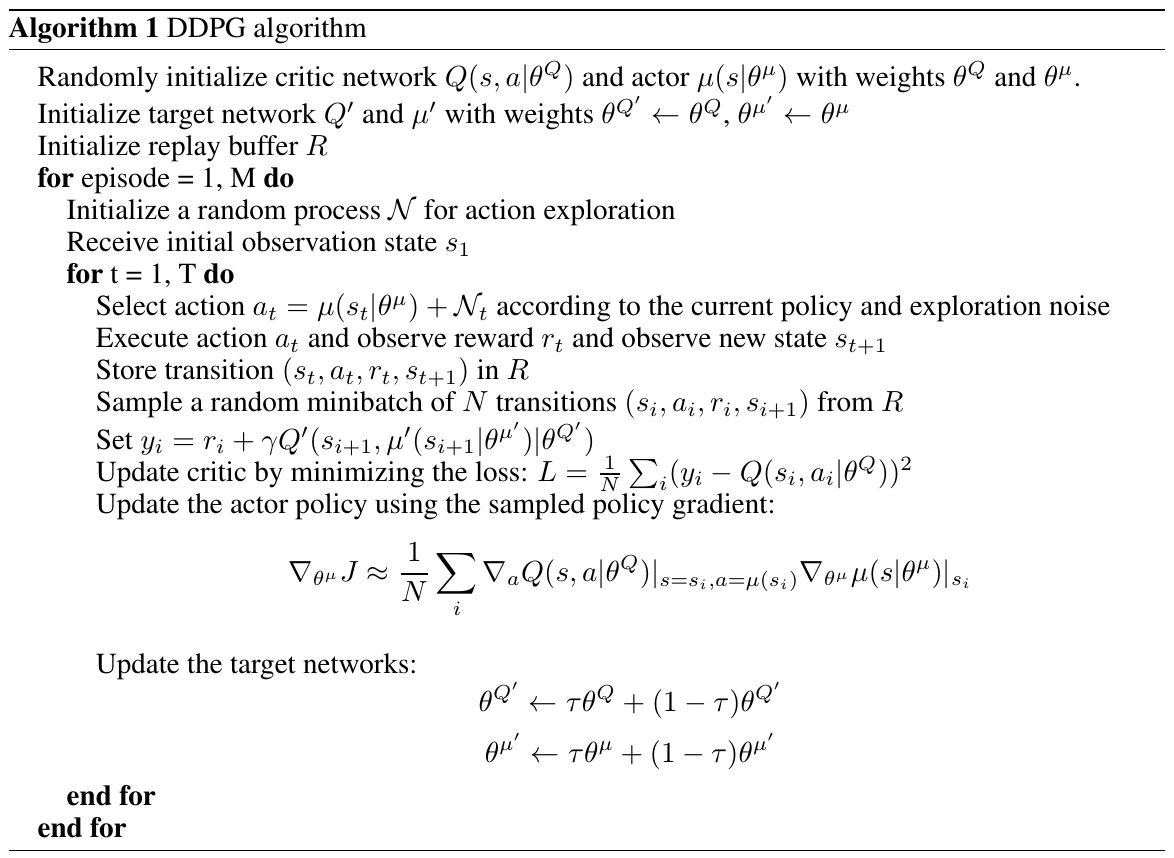
\includegraphics[scale=0.35]{ddpg_algo}
\end{figure}
\end{frame}

\section{Setup}
\frame{\tableofcontents[currentsection, hideothersubsections]}

\begin{frame}
\frametitle{Experiment Setup: Tasks}

\begin{figure}
    \centering
    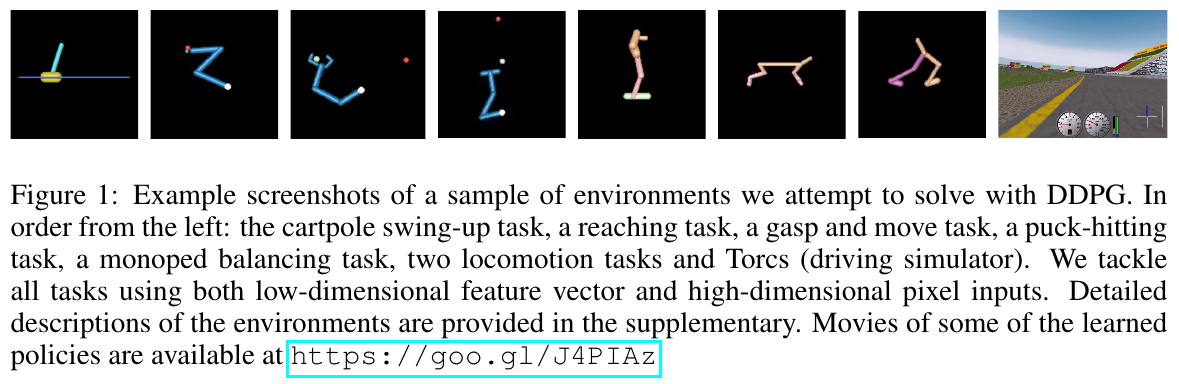
\includegraphics[scale=0.3]{fig_1}
\end{figure}

\begin{itemize}
  \item 20 simulated physics task, including:
  \begin{itemize}
    \item gripperRandom:
    Agent must use an arm with gripper appendage to grasp an object and manuver the object, which
    are initialized in random locations
    % \item reacher3daRandomTarget:
    % Agent is required to move a 7-DOF human-like arm from random starting locations to random target positions.
    \item reacherObstacle:
    Agent is required to move a 5-DOF arm around an obstacle to a randomized target position.
  \end{itemize}
  \item features, both:
    \begin{itemize}
    \item a low-dimensional state description (such as joint angles and positions)
    \item high-dimensional renderings of the environment
  \end{itemize}
\end{itemize}

\end{frame}

\begin{frame}
\frametitle{Experiment Setup: Tasks}

\begin{figure}
    \centering
    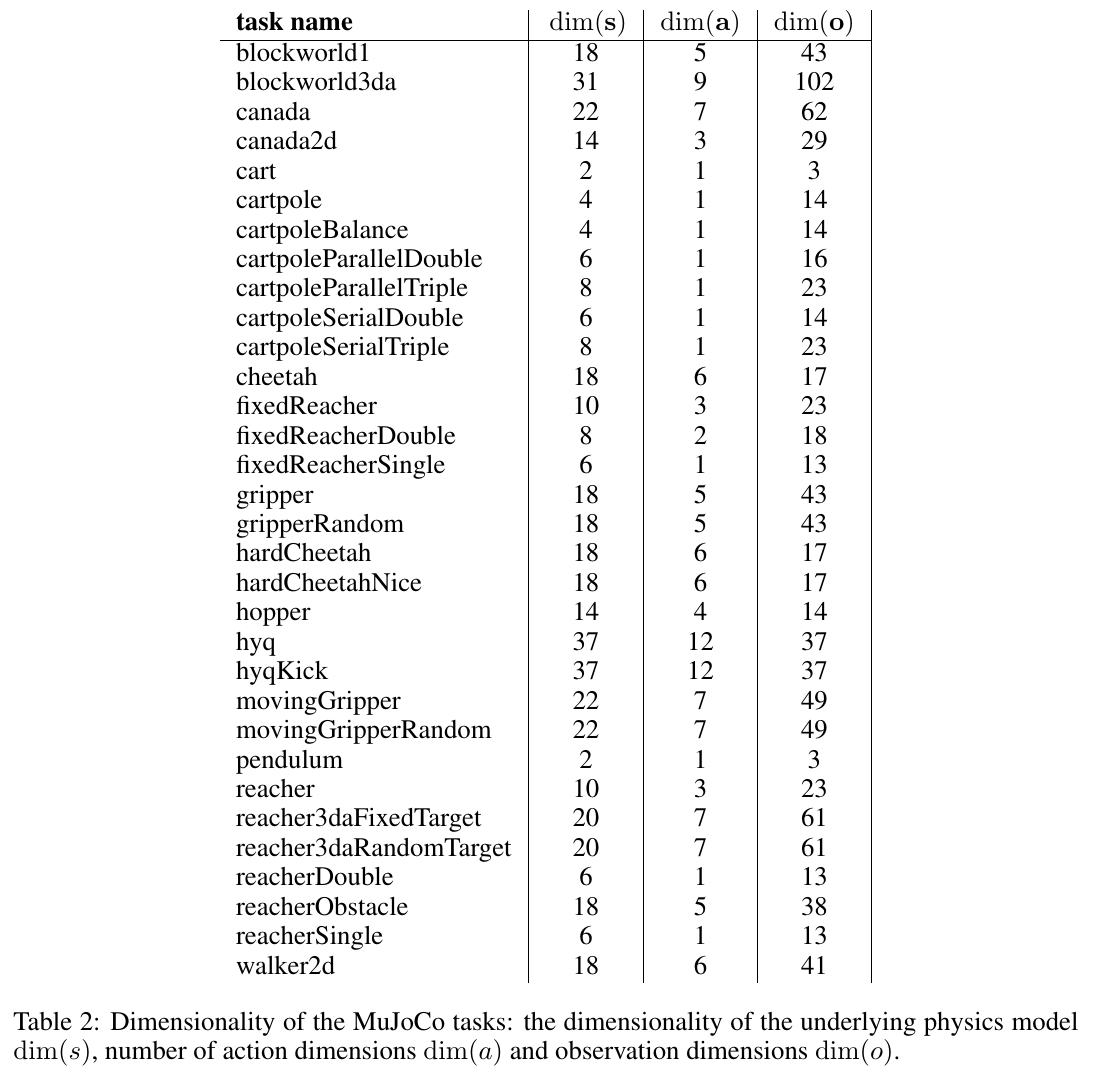
\includegraphics[scale=0.25]{task_dim}
\end{figure}

\end{frame}


\begin{frame}
\frametitle{Experiment Setup: Baseline, Assumptions}

Assumption:
\begin{itemize}
  \item env is MDP, the environment is fully-observed
\end{itemize}

Baseline:
\begin{itemize}
  \item 2 types:
  \begin{itemize}
    \item \textbf{naive policy:} the mean return from a naive policy which samples actions from
    a uniform distribution over the valid action space;
    \item \textbf{iLQG~\cite{Todorov2005}}: a planning based solver with full access to
    the underlying physical model and its derivatives.
  \end{itemize}
  \item normalize baseline scores so that
    \begin{itemize}
    \item \textbf{naive policy}: has a mean score of 0
    \item \textbf{iLQG}: has a mean score of 1
  \end{itemize}
\end{itemize}

\end{frame}


\section{Results}
\frame{\tableofcontents[currentsection, hideothersubsections]}

\begin{frame}
\frametitle{Results: Performance after training}
\begin{figure}
    \centering
    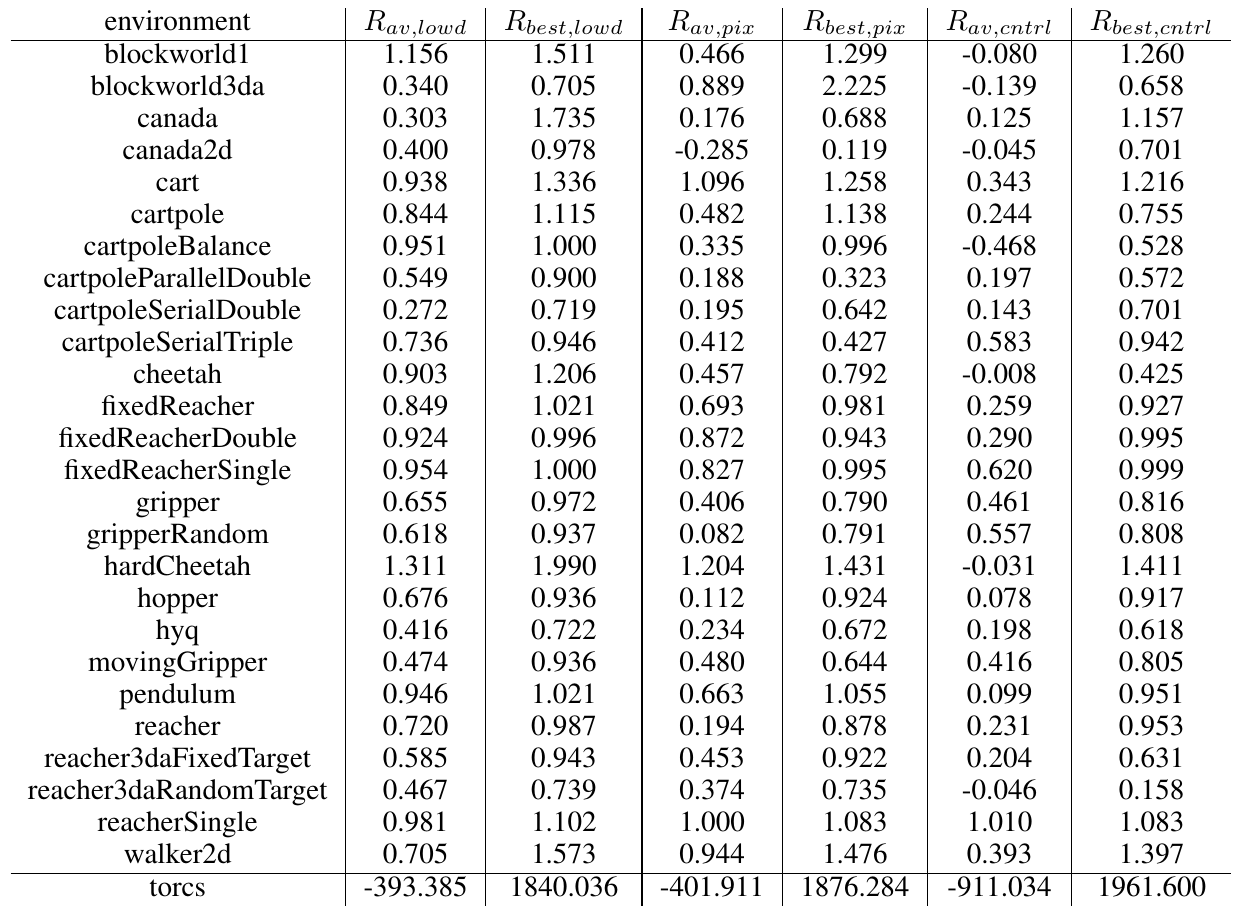
\includegraphics[scale=0.3]{perf_table}
\end{figure}
\end{frame}

\begin{frame}
\frametitle{Results: Estimated Q values}
% \begin{figure}
%     \centering
%     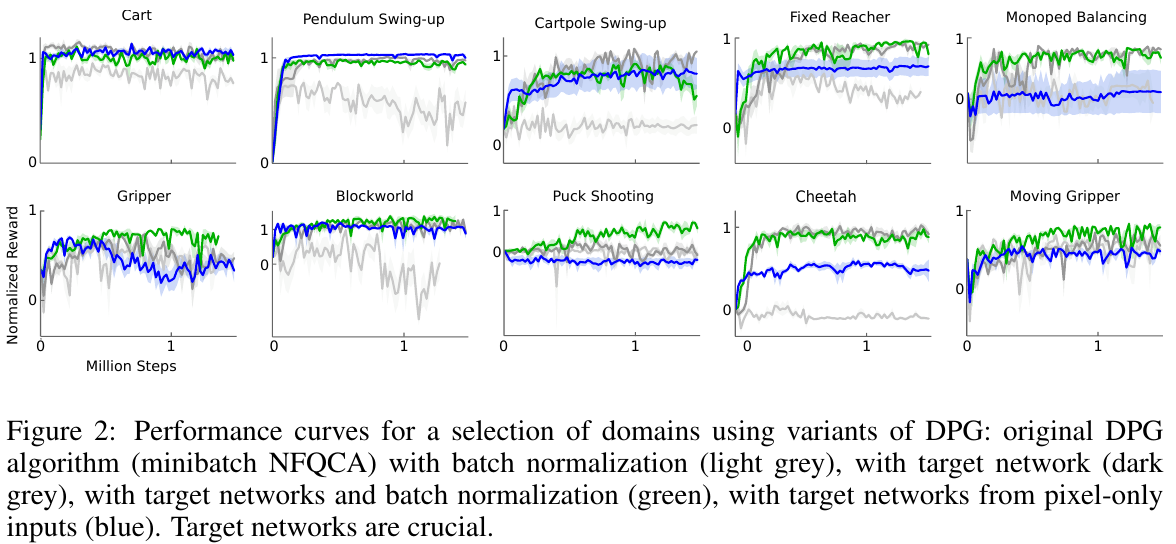
\includegraphics[scale=0.3]{fig_2}
% \end{figure}

\begin{figure}
    \centering
    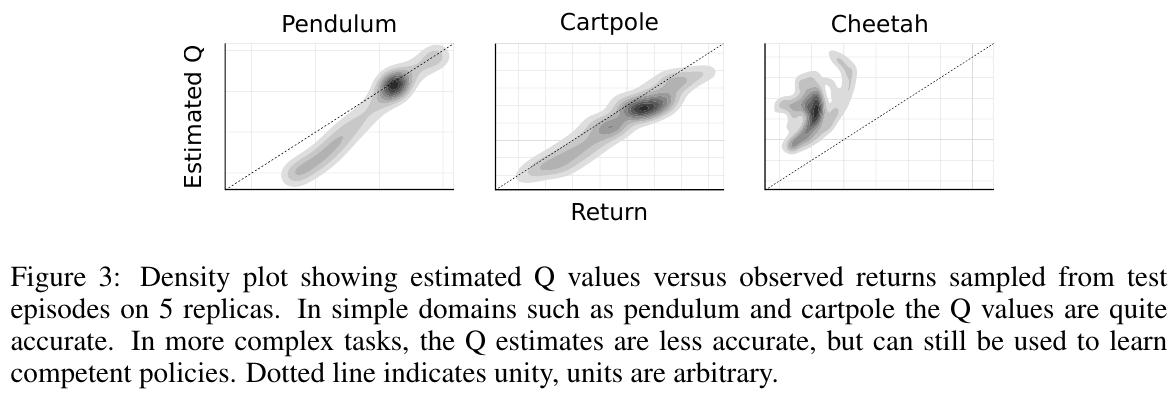
\includegraphics[scale=0.35]{fig_3}
\end{figure}

See: video!
\end{frame}

% \begin{frame}
% \frametitle{Result List}

% \begin{itemize}
%   \item able to find policies whose performance is competitive with those found by a planning algorithm with full access to the dynamics of the domain and its derivatives.
%   \item for many of the tasks the algorithm can learn policies “end-to-end”: directly from raw pixel inputs.
% \end{itemize}

% Surprisingly, in some simpler tasks, learning policies from pixels is just as fast as learning using the low-dimensional state descriptor. This may be due to the action repeats making the problem simpler. It may also be that the convolutional layers provide an easily separable representation of state space, which is straightforward for the higher layers to learn on quickly.

% \end{frame}

\section{Conclusions}
\frame{\tableofcontents[currentsection, hideothersubsections]}

\begin{frame}
\frametitle{Conclusions}

SGD can directly minimize the risk function
\begin{itemize}
    \item by sampling a point i.i.d from D \textbf{and}
    \item using a subgradient of the loss of the current hypothesis at this point as
    an unbiased estimate of the (sub)gradient of the risk function.
\end{itemize}
\vspace{5mm}

SGD's \textbf{convergence rate} and \textbf{the number of iterations} \\
would guarantee an expected objective of at most $\epsilon$ plus the optimal objective.
\vspace{5mm}

WARN: Skipped (Subsub)sections:\\
\begin{itemize}
    \item any proofs
    \item 14.2.2 Subgradients of Lipschitz Functions
    \item 14.4 Variants
\end{itemize}

\end{frame}


\section{My Current Work}
\frame{\tableofcontents[currentsection, hideothersubsections]}

\begin{frame}
\frametitle{My current work: Interest}

\begin{figure}
    \centering
    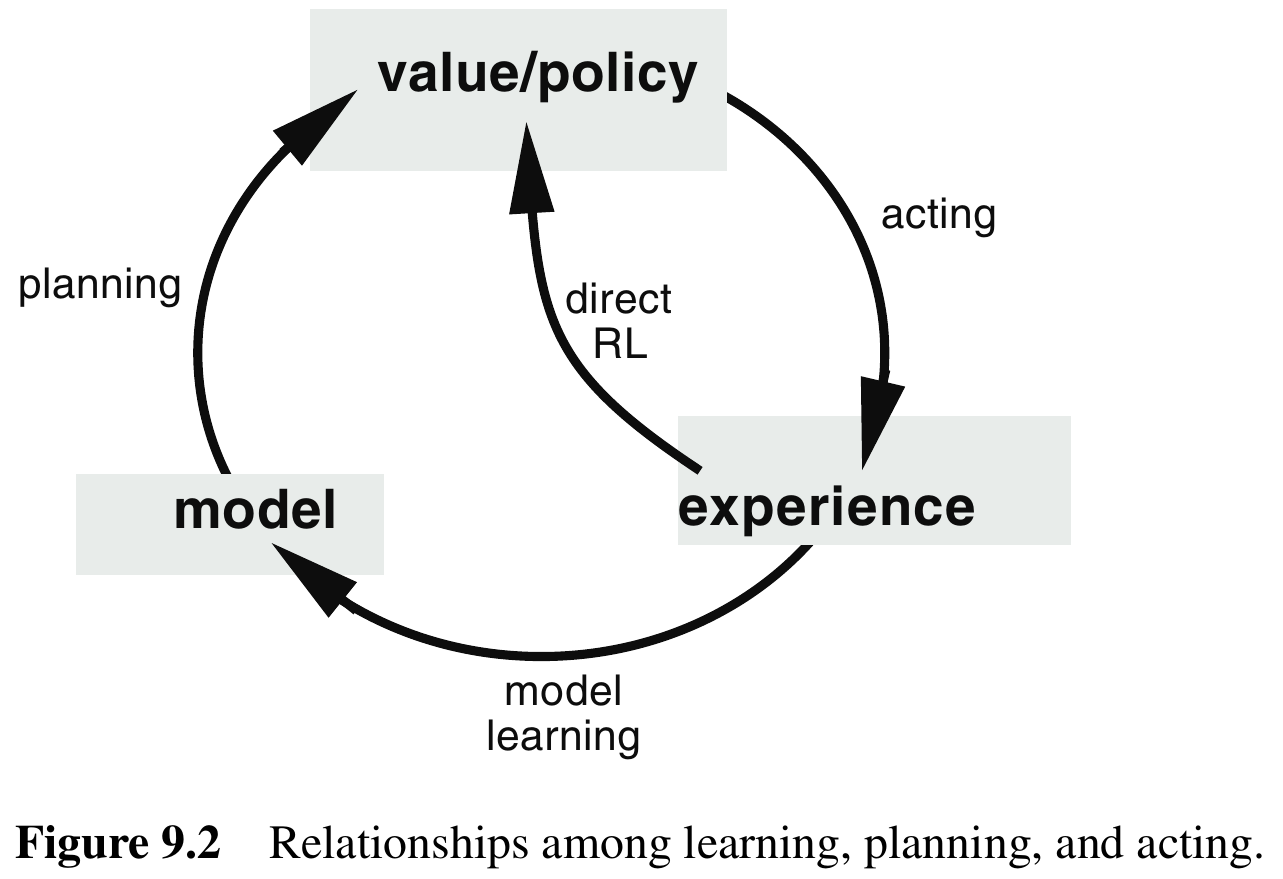
\includegraphics[scale=0.20]{learningplanning_arch}
\end{figure}

Interests, lack of ideas still :(
\begin{itemize}
  \item interaction of model-based and model-free RL, continuous control,
  deeply bayesian RL for POMDPs,
  \item physics-intensive tasks with real robots
\end{itemize}
\end{frame}

\begin{frame}
\frametitle{My current work: On going}
\begin{itemize}
  \item playing around with sim timestep, case: grasping
  \item movodemo, case: pickandplace
\end{itemize}
\vspace{5mm}

Enjoy: some videos!
\end{frame}

% \begin{frame}
% \frametitle{Interests: more detail}
% Nuts and Bolts Task:
% Assumed that the robot has already been trained to recognize, want, grasp, and eat cookies.
% The cookies in this task are within cages, and the cage covers are locked with nuts and bolts.
% The robot must learn to use a wrench and his fingers to remove the cover and get the cookie.
% \end{frame}

% Practical :
% \begin{itemize}
%   \item grasping, using tools,
%   e.g.  Nuts and Bolts Task:
%   \item navigation among movable obstacles
%   (motion planning with minimal collisions)
%   \item (physics) games, e.g
%   car racing, block stacking (simplified Tummple, Jenga)
% \end{itemize}

\begin{frame} [allowframebreaks]
\frametitle{References}
{\tiny
\bibliographystyle{apacite}
\bibliography{ref}
}
\end{frame}

\begin{frame}
\Huge{\centerline{Discussion time and thank you.}}
\end{frame}

%%%%%%%%%%%%%%%%%%%%%%%%%%%%%%%%%%%%%%%%%%%%%%%%%%%%%%%%%%%%%%%%%%%%%%%%%%%%%%%

\end{document}
